%!TEX root = ../thesis.tex
\section{Abordagens à previsão de defeitos}

Foram já exploradas algumas abordagens para a predição da qualidade do código. Salientam-se neste capítulo algumas técnicas como \emph{BugCache}, \emph{FixCache} e \emph{Buggy Change Classification}, que são técnicas que se incluem no tipo de abordagem que pretendemos seguir (\emph{change log}) e que permitem, em conjunto com outras técnicas, otimizar a localização dos defeitos.

\subsection{\emph{BugCache/FixCache}}

Com base na premissa de que as falhas nunca ocorrem isoladamente e que portanto onde existe um defeito existem outros, o \emph{BugCache} cria uma lista de componentes onde a probabilidade de conterem erros é elevada, com base na análise em todo o histórico de alterações do projeto.

Este algoritmo destaca-se pela sua precisão, conseguindo uma exatidão de 73 a 95\% quando usado com uma granularidade ao nível do ficheiro, sendo portanto o melhor até à data \cite{Kim2006}.

Os defeitos são identificados por ordem temporal e adicionados à lista. Quando esta lista atinge o tamanho máximo, os componentes vão sendo removidos de acordo com o método de substituição escolhido. Existem diversos métodos que utilizam diferentes métricas como última utilização (\emph{Least Recent Used - LRU}), número de defeitos recentes e número de alterações recentes \cite{Kim2006}.

Conclui-se com este algoritmo que \cite{Kim2006}:
%
\begin{itemize}
	\item Caso tenha sido introduzido um defeito, há uma tendência para serem introduzidos mais defeitos em breve. (\emph{temporal locality})
	\item Caso um componente tenha sido acrescentado ou modificado recentemente este tem uma maior probabilidade de ser defeituoso (\emph{changed-entity locality}, \emph{new-entity locality})
	\item Caso um componente tenha introduzido um erro, os componentes ligados mais diretamente a este introduzirão também erros no futuro (\emph{spatial locality})
\end{itemize}

A diferença entre o \emph{BugCache} e o \emph{FixCache} é o momento em que cada um atualiza a lista. Sendo que o primeiro atualiza a lista quando um defeito é introduzido, o segundo atualiza apenas quando o erro é corrigido. Devido a esta diferença a implementação do \emph{FixCache} torna-se mais fácil.

\subsection{\emph{Buggy Change Classification}}

\emph{Change Classification} tem uma abordagem fundamentalmente diferente e tem um objetivo também distinto. O \emph{Change Classification}, com recurso a técnicas de \emph{Machine Learning} e às informações disponíveis quanto a erros anteriores, é capaz de prever se uma alteração introduziu ou não um novo defeito. Esta previsão é feita com um rigor muito elevado de 78\% \cite{Whitehead2008}.

Numa primeira fase, todas as alterações feita até ao momento são classificados como \emph{buggy} ou \emph{clean}. Com esta classificação feita e com a extração de dados para cada também concluída, procede-se à criação de um modelo através do \"treino\" de um algoritmo de classificação.

O tipo de dados usados dividem-se em sete grupos: métricas de complexidade, código adicionado, código removido, nome do ficheiro e diretório, novo código e meta-dados \cite{Whitehead2008}.

Tanto \emph{Support Vector Machine} (SVM) como \emph{Naïve Bayes} foram usados no estudo, tendo sido o classificador feito com recurso a SVM aquele que apresentou melhores resultados \cite{Whitehead2008}.

\subsection{Data-Augmented Software Diagnosis} \label{subsec:elmishali}

A different approach that also aims to help predict the location of software faults is Data-Augmented Software Diagnosis \cite{Elmishali}.

Model-based and spectrum-based approaches are able to identify faulty components with high precision and recall, but there is still room for improvement and since most projects use some kind of Version Control Software (VCS), there is a big amount of information that is not used. This opportunity is the foundation of the approach.

Barinel assumes that the defect probability, known as the prior, of every component is uniform, $0.001$. However, this approach proved it is possible to optimize Barinel results for Java projects by leveraging information about the project and supervised machine learning algorithms to predict the real component's defect probability.

First, healthy and faulty components are identified across the entire project's history according to Bug Trackers. For each component, a list of features, which is not specified, is extracted. The list is composed of traditional and object-oriented software complexity metrics, such as number of lines of code and cohesion, and values extracted from the software change history, like lines added or removed in last version and age of the file.

With the help of a supervised machine learning algorithm (either Random Forest, J48 or Naive Bayes) a model is created and used to classify each component in the project as healthy or buggy. The confidence that a component is faulty is then used as prior.

Experimental results revealed an increment both on precision and recall, see Figure \ref{fig:elmishali}. However, the solution was tested just on one project.
%
\begin{figure}%
    \centering
    \subfloat[Precision]{{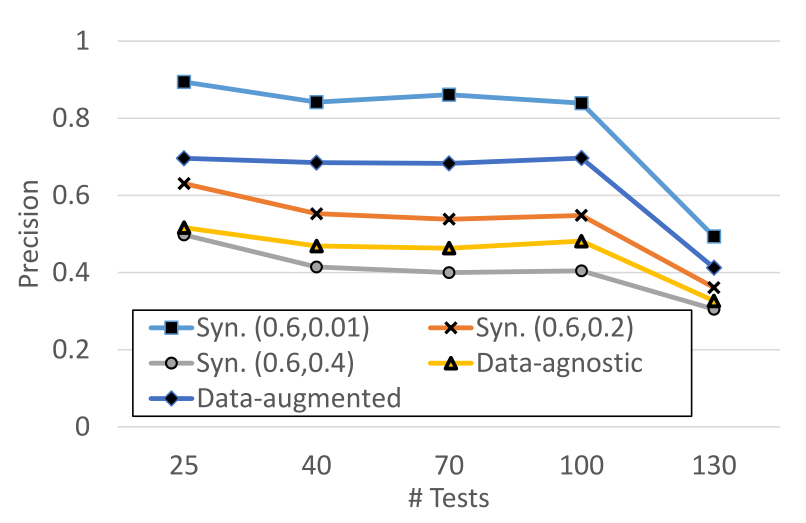
\includegraphics[width=0.4\textwidth]{elmishali-precision} }}%
    \qquad
    \subfloat[Recall]{{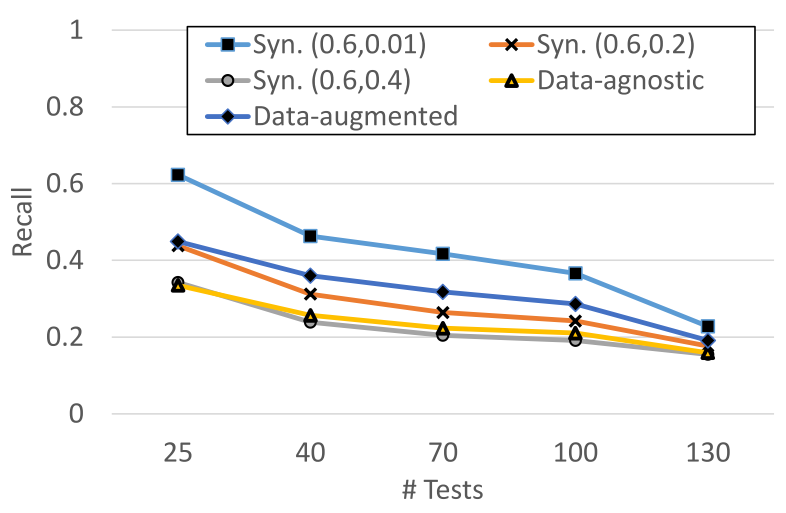
\includegraphics[width=0.4\textwidth]{elmishali-recall} }}%
    \caption{Diagnosis accuracy as a function of \# tests given to the diagnoser}%
    \label{fig:elmishali}%
\end{figure}
